\documentclass{article}

\usepackage[french]{babel}
\usepackage[utf8]{inputenc}
\usepackage[T1]{fontenc}
\usepackage{graphicx}
\usepackage{amsmath,amsfonts,amssymb}
\usepackage[margin=3cm]{geometry}

\begin{document}
\pagestyle{empty}



\section{Étiquettes et bonbons}

\textbf{Énoncé}: Voici trois bocaux de bonbons. Il y a deux sortes de bonbons, des bonbons à la fraise et des bonbons à l'orange. Il y a un bocal avec uniquement des bonbons à la fraise, un bocal avec uniquement des bonbons à l'orange, et un bocal avec des bonbons à la fraise et des bonbons à l'orange (mais on ne sait pas combien de chaque). Ces bocaux sont opaques, on ne peut donc pas voir quelle sorte de bonbons ils contiennent sans en gouter un ou en lisant l'étiquette en dessous du bocal. \\

\begin{center}
	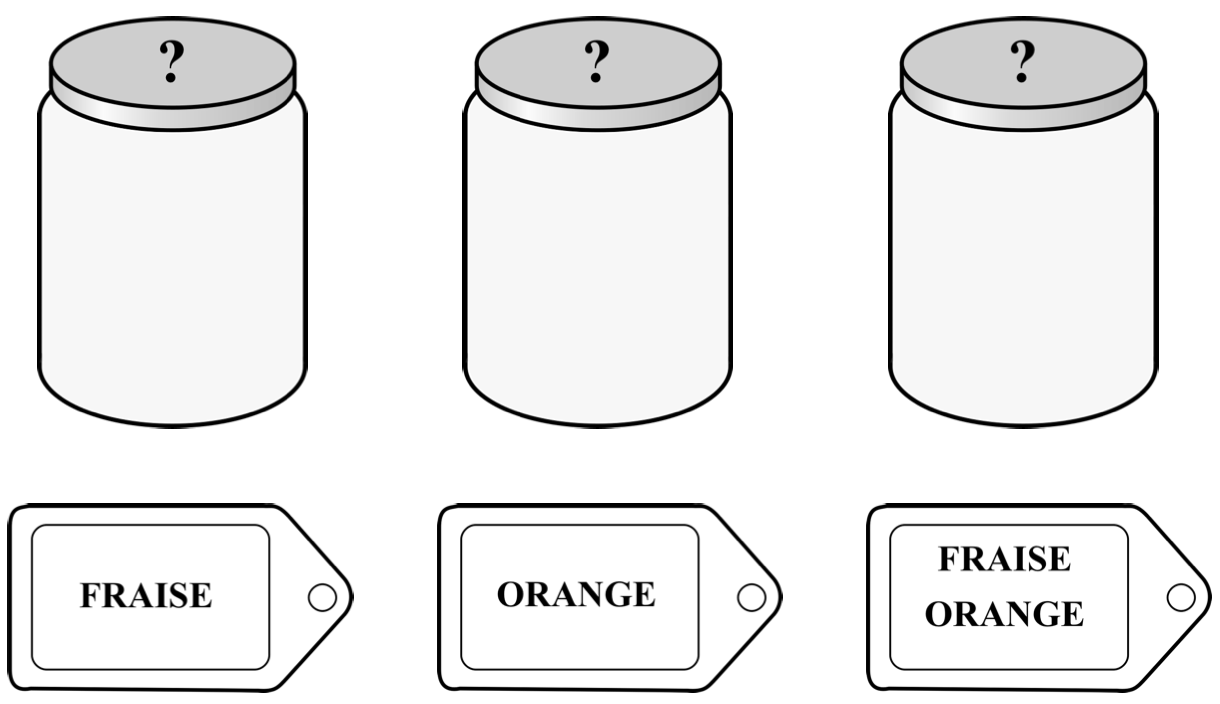
\includegraphics[scale=0.5]{Figures/Etiquettes.png} 
\end{center}

\textbf{Problème }: quelqu'un a mélangé toutes les  étiquettes de ces bocaux ! aucune  étiquette n'est à la bonne place. Combien de bonbons minimum faut-il de manger pour savoir le contenu de chaque bocal ? \\


   


  
\section{Auto-référence} 

\begin{center}
	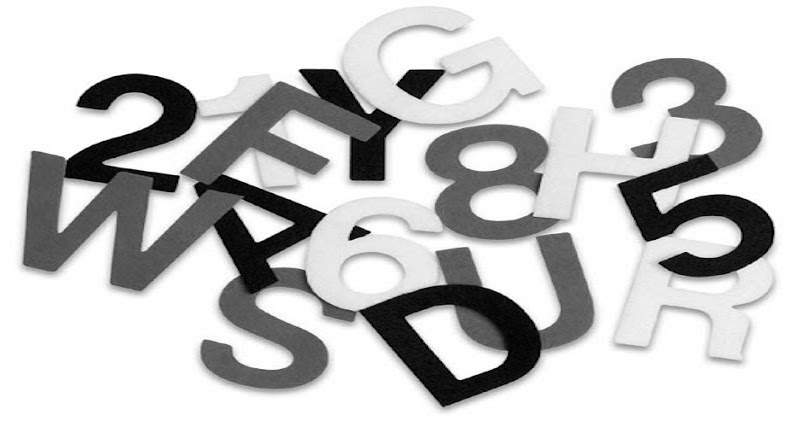
\includegraphics[scale=0.375]{Figures/lettres} 
\end{center}

\hspace{3cm}

\textbf{Énoncé }: Par quel nombre (de deux chiffres), écrit en lettres, faut-il compléter la phrase suivante pour qu'elle soit vraie ? \\

\begin{center}
	\textbf{Dans cette phrase on peut dénombrer ... lettres. } \\
\end{center}

  

  
\newpage  
\section{Les personnes dans les escaliers}

\textbf{Énoncé}: Quatre personnes sont placées dans des escaliers. Elles regardent toutes vers le bas. Entre la personne 3 et la personne 4, un mur est placé. Donc les personnes 1, 2 et 3 ne peuvent pas voir la personne 4. Elles portent toutes un chapeau qui est soit de couleur noire, soit de couleur blanche. L'ordre est comme indiqué dans le dessin : noire, blanche, noire, blanche. \\

\begin{center}
	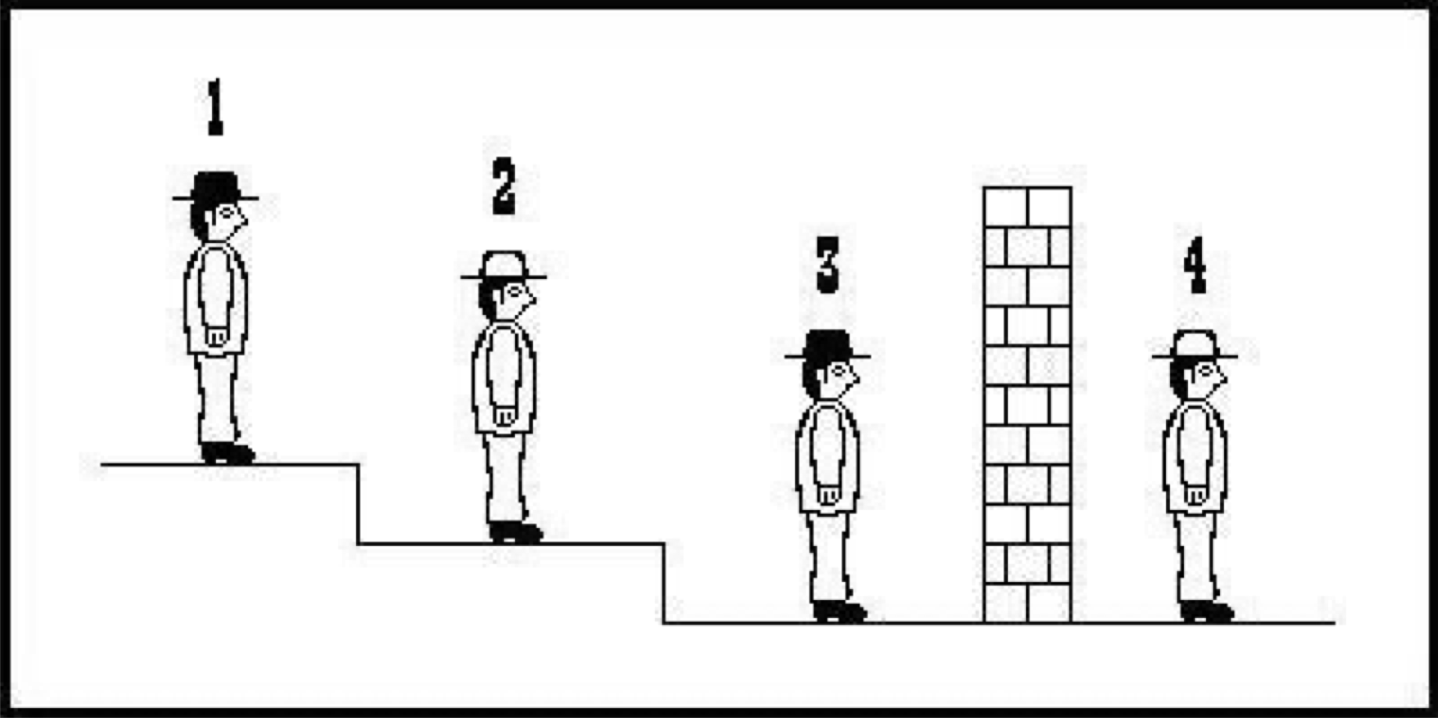
\includegraphics[scale=0.45]{Figures/Bonhommes.png} 
\end{center}

\textbf{Problème }: on demande alors aux personnes : "qu'elle est la couleur de ton propre chapeau ?". Les personnes savent seulement qu'il y a deux chapeaux blancs et deux chapeaux noirs. Il ne peuvent pas bouger, ni se retourner, ni communiquer. Si une des personnes devine la couleur de son chapeau, elle doit crier : "moi, je connais la couleur de mon chapeau !"
Quelle personne est la première à crier "moi, je connais la couleur de mon chapeau !"?

 
\section{Traversée du pont }

\textbf{Énoncé} : Maryam Mirzakhani, Grigori Perelman, Alexander Grothendieck et Karen Uhlenbeck reviennent du donjon perdu et retournent au village. Lorsque l'équipe arrive au pont qu'elle a traversé le matin même, il fait nuit noire. A l'aller le matin, ils ont traversé le pont une personne à la fois. Grigori a traversé le pont en 1 minute, Karen en 2 minutes, Maryam en 5 minutes et Alexander en 10 minutes. Malheureusement il est impossible de traverser sans torche et il ne leur en reste plus qu'une seule qui s'éteindra dans 17 minutes. De plus, le pont ne supporte le poids que de 2 personnes à la fois. Il est nécessaire de faire des allers-retours pour ramener la torche aux personnes qui n'ont pas encore traversé. \\

\begin{center}
	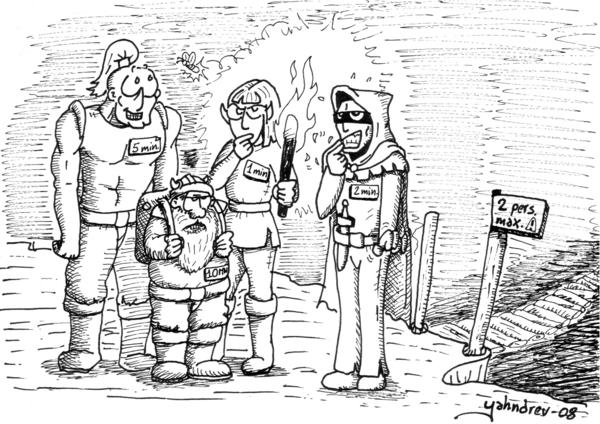
\includegraphics[scale=1.25]{Figures/traverser} 
\end{center}

\textbf{Problème }: Comment cette équipe arrivera-t-elle à traverser le pont ? \\   
   
  
 
  
  
 %%-------------------------------------------------%%     
 %%-------------------------------------------------%% 
 %%-------------------------------------------------%% 
 %%-------------------------------------------------%% 
 %%-------------------------------------------------%% 
 %%-------------------------------------------------%% 
 %%-------------------------------------------------%% 

%\hrule
%\hspace{3cm}
\newpage  



\textbf{Solution 1 } : Comme les  étiquettes sont toutes mal placées, la boite de "F \& O" est soit F soit O. Donc premier coup : on pioche dans le bocal F\& O. Sans perdre généralité, on suppose que c’est F. De plus, le bocal de "F" est soit FO soit O et le bocal de "O" soit F soit FO. Or, "F\& O" est F, donc "O" est forcément FO et ainsi "F" est O. Finalement, 1 seul coup est nécessaire ! \\




\textbf{Solution 2} : Soit N le nombre total de lettres. Sans le chiffre  écrit, il y a déjà $N = 37$ lettres. On aura donc au moins "trente -..." donc au moins 6 lettres en plus. On dépasse donc les 40 lettres, donc $N > 40$. Le mot "quarante" a 8 lettres, ce qui fait $N > 45$. Or, "quarante-cinq" donne $N = 49$, "quarante-six" donne $N = 48$, "quarante-sept" donne $N = 49$, "quarante-huit" donne $N = 49$, "quarante-neuf" donne $N = 49$. \\

\textbf{Solution 3 } : C'est le personnage 2. En effet, le personnage 1 ne peut pas connaitre la couleur de son propre chapeau, et il remarque que les personnage 2 et 3 ont des chapeaux de couleurs différentes. Ainsi le personnage 1 reste silencieux, et le personnage 2 en déduit que son chapeau n'est pas de la même couleur que le chapeau du personnage 3. \\

\textbf{Solution 4} : Grigori et Karen traversent le pont : 2 min. Grigori revient : 1 min. Maryam et Alexander traversent le pont : 10 min. Karen revient : 2 min. Grigori et Karen traversent le pont : 2 min. \\



%\section{Ordre et somme  (un peu d'additions)}
%
%\textbf{Énoncé} : On cherche 4 chiffres, ordonnés de manière strictement croissante. $$...<...<...<...$$
%
%En collant les deux plus petits, on obtient un premier nombre, et en collant les deux plus grands on obtient un second nombre. On souhaite que le premier nombre soit la moitié du second.  Par exemple :
%$$ 2<3<4<6,  \text{ et } 23 = \frac{46}{2}$$
%Mais ce n'est pas tout, on veut également que la somme des deux nombres soit plus grande que 100. Dans notre exemple, cela ne fonctionne pas car
%$ 46 + 23 = 69 < 100. $ \\
%
%\textbf{Problème }:  Quels sont les 4 chiffres qui sont solution ? \\
 
% \textbf{Solution 2} :  $3 < 4 < 6 < 8, \text{ et } 34+ 68=102 > 100$ \\
 
 
 
%\textbf{Solution 4 } : Pour le plat de résistance, on met 2 tranches sur la plaque. Après 5 minutes on enlève la 2 ème, on met la 3 ème à cuire et on retourne la 1 ère. Après autre 5 minutes on enlève la 1ere qui est cuite, on remet la 2 ème et on retourne la 3 ème. Puis on attend encore 5minutes, ce qui fait 15 minutes en tout. \\


\end{document}